\section{Results}\label{sec:results}
% \vicki{You need to explain the experimental setup first.}
% MDH: This was explained in Contribution, but I've added another paragraph there to
% explain each step. Is there anything else I need to add?

\subsection{Mechanism Combinations}\label{subsec:mechanism-combinations}
The absolute mean error by coordination mechanism per voting mechanism is graphed in
\autoref{fig:vm-col-cm-hue-error-as-percent-of-space-abs-mean}.
% \vicki{We need to know how the proxies work  You gave us several choices, but we can't
% map them to the choices shown here.  Also, how many total voters are there? }
% MDH: I've added this to the `experimental setup' paragraph.
There are a few trends that are immediately identifiable.
First, error unsurprisingly increases as the number of inactive agents increases.
This is true with two notable exceptions: first, the Active Only/Median
mechanism combination has a somewhat sawtooth shape.
This is due to the Median mechanisms always choosing a specific agent's preference
instead of aggregating to some more preferential in-between value.

The second exception is that Mean mechanism consistently dips when all but one agent
become delegators.
This is because we take the mean of the constituents and the proxy, then apply the
voting mechanism on the set of proxy-constituent votes.
Since there is only one proxy-constituent vote, the result is the vote itself.
Essentially, the coordination mechanism replaces the voting mechanism.

We can also see the Mean and Median coordination mechanisms generally yield similar
amounts of error.
In particular, when either of these mechanisms is combined with the Mean voting
mechanism the results are very similar to when all agents are active and able to vote.

Notably, the Expert coordination mechanism works worse than the others as the number
of delegators reaches a significant portion of the population.
In particular, the Expert mechanism tracks nearly identically to Active Only when
using the Midrange voting mechanism.
Depending on the use case, this may or may not be beneficial.
If we are attempting to find the best result for all agents, this mechanism may yield
undesirable results.
However, if we are attempting to exploit the experts experience, as described
by~\cite{Miller1969}, this error could actually be considered the improvement over
the original result.
This is because the experts were able to influence and change the vote, presumably
bringing it closer to what their expertise dictates.
Nevertheless, when the number of delegators is low, the Expert mechanism works
similarly to the other coordination mechanisms.

\begin{landscape}
    \begin{figure}[p]
        \centering
        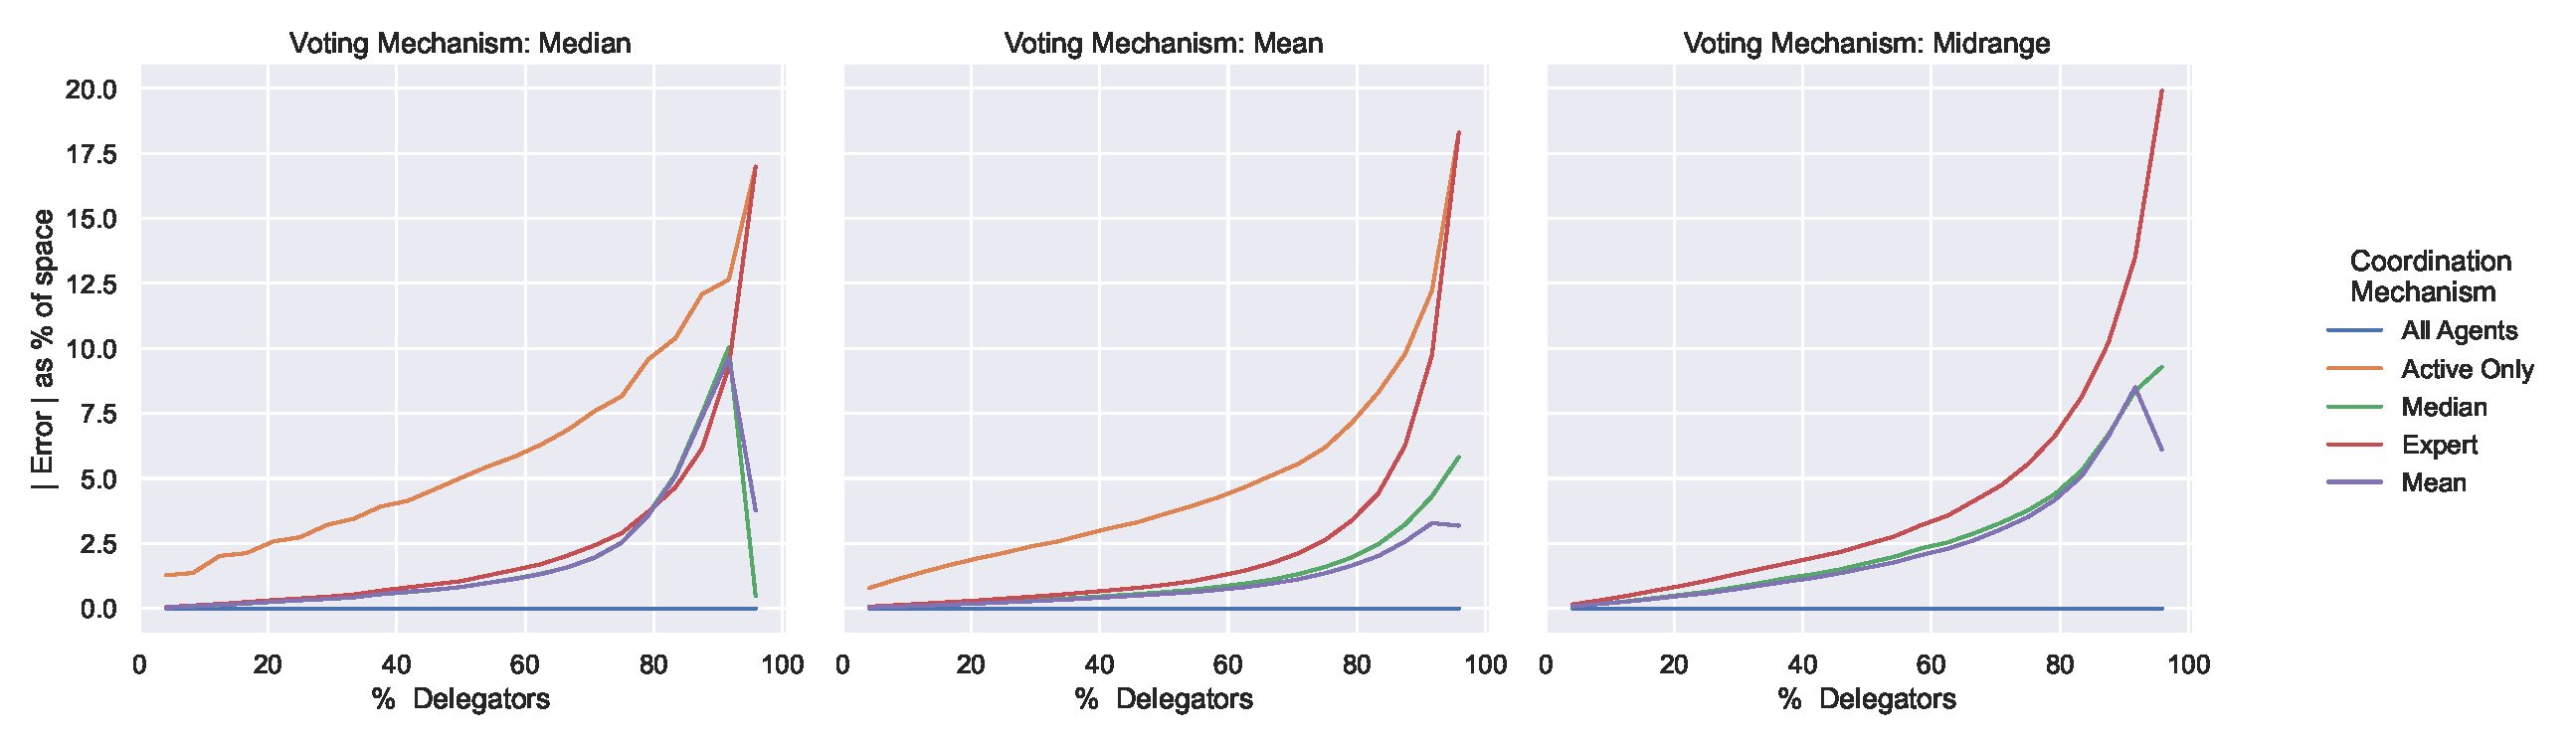
\includegraphics[scale=0.55]
        {content/chapter2/figures/vm_col_cm_hue_error_as_percent_of_space_abs_mean}
        \caption{
            The absolute mean error as a percent of the preference space by
            coordination mechanism per voting mechanism.
            `Error as a percent of the preference space' means the error divided by
            the total size of the preference space.
            Note All Agents represents when all agents are voting, meaning no proxy
            voting is used and all agents are present.
            Similarly, Active Only represents when proxy voting is not used and not
            all agents are present, and when proxies lose their constituents.
            There are 24 total agents.
        }
        \label{fig:vm-col-cm-hue-error-as-percent-of-space-abs-mean}
    \end{figure}
\end{landscape}

Importantly, it is clear that using proxy voting, regardless of the mechanisms used,
is better than losing information by not allowing inactive agents to vote in any way.

\subsection{By Distribution}\label{subsec:results-distribution}
\autoref{fig:distribution-error-as-percent-of-space-abs-mean} shows
the absolute error as a percent of the preference space by coordination mechanism for
each voting mechanism and preference distribution.
\autoref{fig:distribution-different-scale-error-as-percent-of-space-abs-mean} shows
the same graphs, but with a different scale for each plot to more easily see the shape.
Additionally, each graph is zoomed in for readability
in~\autoref{apx:error-by-dist-zoomed}.

\begin{figure}[p]
    \centering
    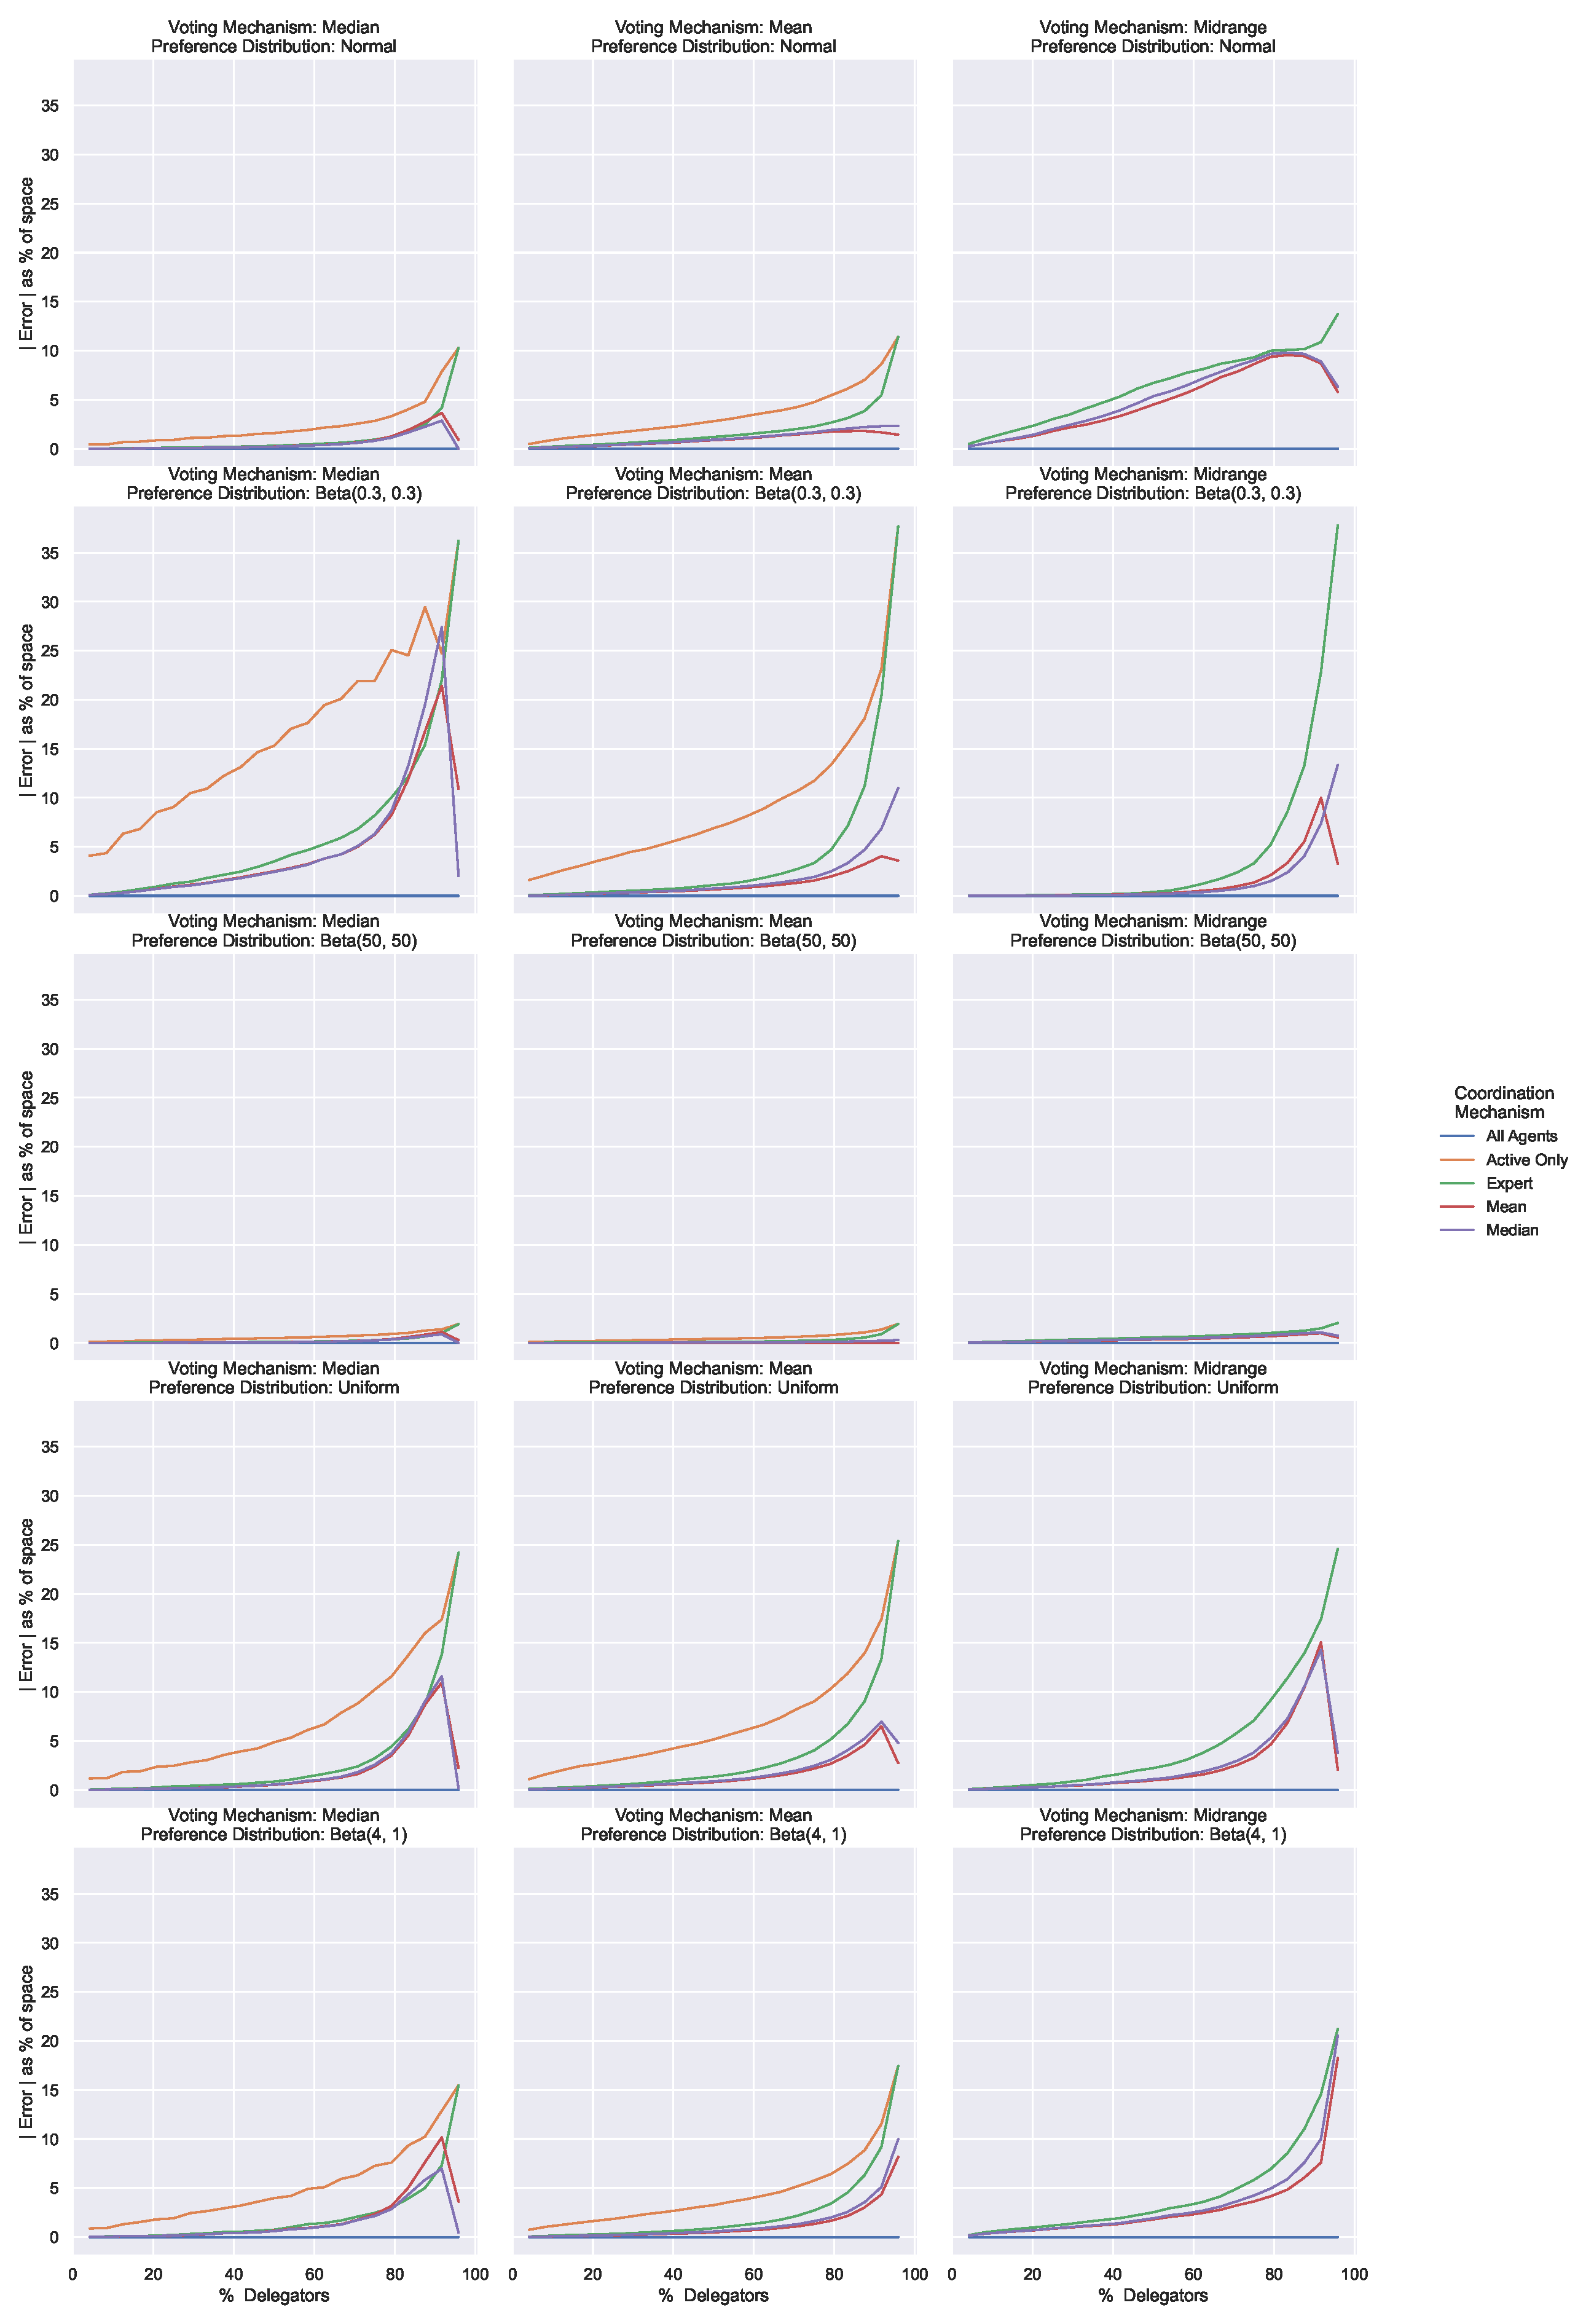
\includegraphics[scale=0.30]
    {content/chapter2/figures/distribution_error_as_percent_of_space_abs_mean}
    \caption{
        The absolute error as a percent of the preference space by coordination
        mechanism for each voting mechanism and preference distribution.
        There are 24 total agents.
    }
    \label{fig:distribution-error-as-percent-of-space-abs-mean}
\end{figure}

These plots show the increase in error is consistent regardless of the mechanisms or
distributions used.
Mean and Median show a similar amount of error, while Expert shows slightly more
except for near the end and when using the Midrange voting mechanism.
Interestingly, this seems to indicate again that it does not matter how you do proxy
voting so long as it is done.
Additionally, it should be noted the mechanisms perform well on most preference
distributions, including the asymmetrical distribution \betadistribution{4}{1}.

Unfortunately, while the error for other distributions is relatively similar,
\betadistribution{0.3}{0.3} yields considerably more error and starts accumulating
this error earlier.
\betadistribution{0.3}{0.3} represents a highly polarized topic, with its probability
density function (PDF) having large spikes at either end of the preference space.
This would indicate that proxy voting, while it is still better than active-only
voting, does not work quite as well when agents have stronger, opposing opinions.

For the median mechanism voting mechanism, this makes sense.
The median will most often be the preference of a specific agent, instead of some
value in between.
As such, the result will often be in one of the spikes in the PDF, since that is
where the majority of the agents' preferences will be, yielding higher error than when
using the Mean or Midrange voting mechanisms.

With the other voting mechanisms, the error is similar to other distributions using
the same mechanisms until the vast majority of the agents are inactive.
The increase in error is because as more agents go inactive there are fewer agents able
to serve as proxies, and so there may not be as desirable of a proxy to represent
each agent.

While it is still more beneficial to use proxy voting than not in these polarized
cases, agents should make an extra effort to participate in-person to ensure their
voice is heard.

\subsection{Preference Change}\label{subsec:results-shift}
\autoref{fig:abs-diff-from-preference-change-error-as-percent-of-space-abs-mean} shows
the difference between `worst case' preference change, where `worst case' means each
agent can change its preference to any value in the preference space after
deliberations.
% \vicki{It seems unrealistic to think there are huge swings in preference.}
% MDH: I agree, but anything less yielded even smaller differences, as stated in the
% next sentence. I can rerun it with smaller changes again, but it would likely yield
% similar results.
Similar experiments were performed that instead restricted the amount the agents
could change their preference to only a portion of the preference space, which
yielded similar graphs, though with an even smaller y-axis scale.

Unsurprisingly, the amount of error increases as more agents become inactive.
However, it is important to note the magnitude of the scale.
The largest difference in error is $\approx 0.35$ of the preference space,
which ultimately is a very small amount.
This minute difference indicates proxy voting is still beneficial when deliberations
and still underway.
This is an extremely powerful advantage for proxy voting, since it allows the system
to maintain the benefits of deliberation while reducing the voting cost for agents.
\vicki{Why is the mid range so erratic?  You would think delegates wouldn't matter that much as you are only considering two of the votes.  Are you averaging over many cases?  The scores seem too volatile to be true expected behavior.}
\begin{landscape}
    \begin{figure}[p]
        \centering
        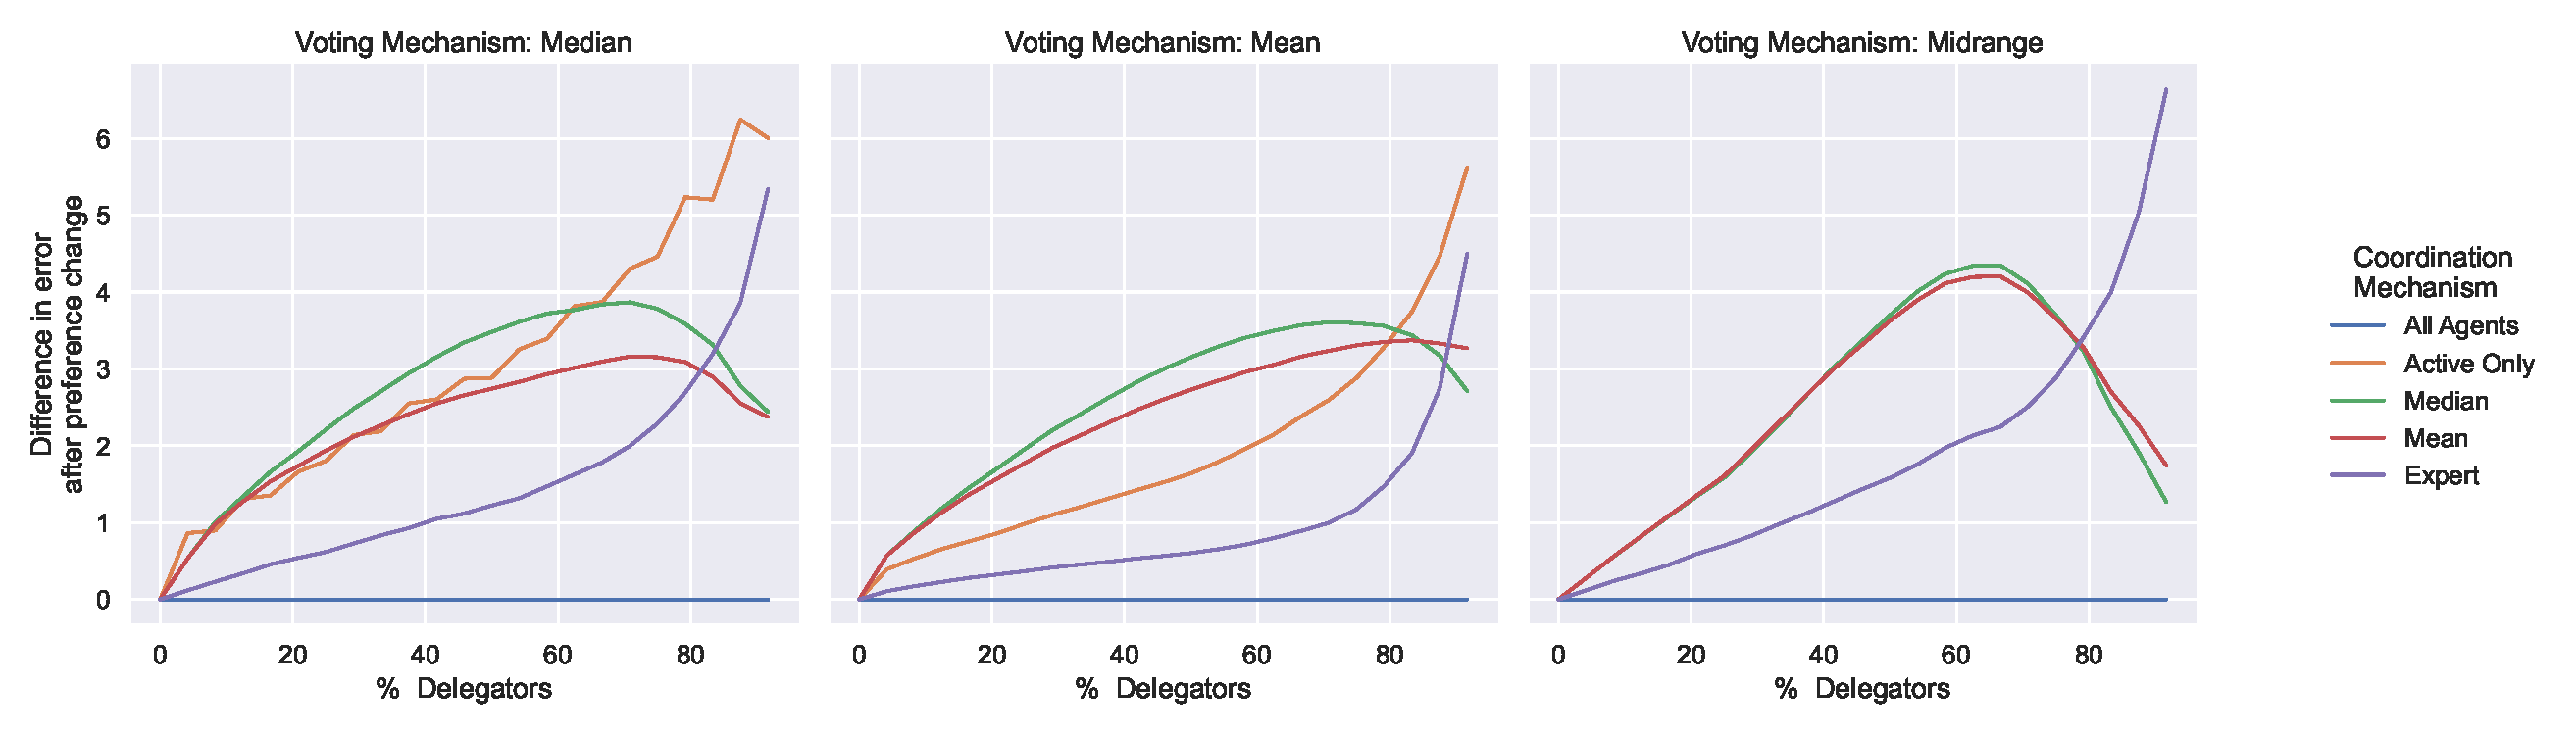
\includegraphics[scale=0.55]
        {content/chapter2/figures/abs_diff_from_preference_change_error_as_percent_of_space_abs_mean}
        \caption{
            The absolute difference in the error produced between without a
            preference change and with a preference change as a percent of space.
            Note the maximum difference is less than 0.5\%.
            There are 24 total agents.
        }
        \label{fig:abs-diff-from-preference-change-error-as-percent-of-space-abs-mean}
        \vicki{Why is the mid range so erratic?  You would think delegates wouldn't matter that much as you are only considering two of the votes.  Are you averaging over many cases?  The scores seem too volatile to be true expected behavior.}
    \end{figure}
\end{landscape}

